%%==================================================
%% ch1.tex for BIT Master Thesis
%% modified by yang yating
%% version: 0.5
%% last update: April 25th, 2017
%%==================================================

\chapter{快速使用指南}
\label{chap:what}

本手册是针对北京理工大学硕士(博士)学位论文~\LaTeX~ 模板BIT-Thesis的使用指南。旨在使同学们通过该使用指南的介绍,能快速掌握使用BIT-Thesis模板编辑符合学校格式要求的硕士(博士)学位论文,并能对~\LaTeX~ 有一定的了解。

\textbf{BIT-Thesis的最新版本以及使用手册地址:}
\begin{center}
\url{https://github.com/BIT-thesis/LaTeX-template}
\end{center}

\section{为什么要用BIT-Thesis}
\label{sec:why}
学位论文通常具有比较严格的格式要求,这是为了方便同行学术交流的起码要求,同时也是科学研究严谨性的体现。然而,由于市场各种排版软件混杂,使用者水平不一,学生对格式的重视程度不够,学生编写标准格式的学位论存在很多问题。BIT-Thesis 为符合北京理工大学硕士(博士)学位论文的LaTeX模板。通过BIT-Thesis模板可以轻松撰写符合学校格式要求的学位论文,学生可避免繁琐的论文格式调整,从而将关注点更多地放在高质量的内容本身。

\section{安装配置环境}
\label{sec:requirements}

\TeX 发展至今日,拥有了众多的发行版。发行版软件合集中包括了各种引擎的可执行程序,以及一些文档类、模板、字体文件、辅助程序等等。

\begin{itemize}
\item windows、linux用户推荐安装TeX Live套装,并更新宏包
\item OSX用户推荐安装Mac TeX
\item 由于CTeX套装所含宏包比较陈旧,可能会导致编译无法通过,故不推荐安装
\end{itemize}

可在对应官方网站上下载安装,也可以使用\textbf{北京理工大学开源软件镜像服务}进行下载(推荐): \url{http://mirror.bit.edu.cn/CTAN},其中
\begin{itemize}
\item TeX Live镜像:\url{http://mirror.bit.edu.cn/CTAN/systems/texlive/Images/}
\item Mac TeX镜像:\url{http://mirror.bit.edu.cn/CTAN/systems/mac/mactex/}
\end{itemize}



\section{快速使用}
\label{sec:process}

安装完TeX套装后,一般而言所需的环境就配置好了。

下面以硕士学位论文模板BIT-thesis-template-master为例,进入BIT-thesis-template-master文件夹。
windows系统点击运行BIT-thesis-run.bat脚本,linux系统以及mac系统请点击运行BIT-thesis-run.sh脚本。脚本会自动运行如图\ref{fig:run} 所示(第一次运行可能需要较长时间,请耐心等待)。打开生成的pdf文档demo.pdf查看模板生成内容。
 
\begin{figure}[!htp]
  \centering
  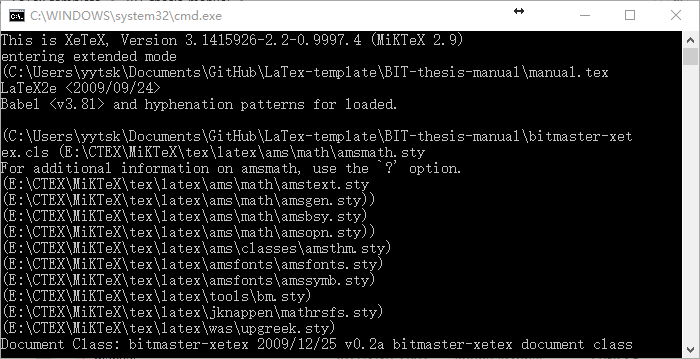
\includegraphics[width=0.85\textwidth]{figures/BIT-thesis-run}
  \caption{BIT-thesis-run.bat脚本运行}
  \label{fig:run}
\end{figure}


\begin{figure}[!htp]
  \centering
  {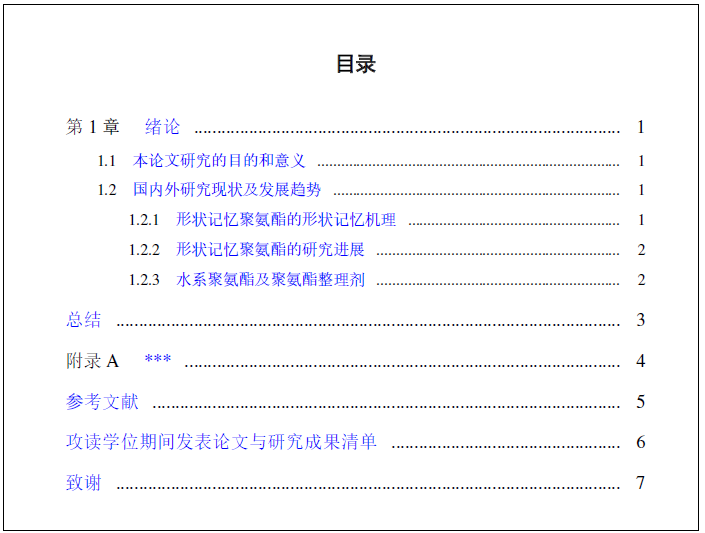
\includegraphics[width=0.85\textwidth]{figures/demo_context}}
  \caption{生成文档demo.pdf的目录}
  \label{fig:demo_context}
\end{figure}

本模板使用~\XeTeX~ 引擎提供的~\XeLaTeX~的命令处理,作用于“主控文档”demo.tex。
由于该模板使用~{{\sc Bib}\TeX}~处理参考文献,构建流程为 \textbf{XeLaTeX$\rightarrow$ BibTeX $\rightarrow$ XeLaTeX$\rightarrow$ XeLaTeX}。完整的处理流程是:

{\color{blue}
\begin{enumerate}
\item[] ~\verb|xelatex -no-pdf --interaction=nonstopmode demo|
\item[] ~\verb|bibtex demo| 
\item[] ~\verb|xelatex -no-pdf --interaction=nonstopmode demo|
\item[] ~\verb|xelatex --interaction=nonstopmode demo|
\end{enumerate}}

运行bibtex的时候会提示一些错误,可能是~{{\sc Bib}\TeX}~对UTF-8支持不充
分,一般不影响最终结果。加入~\verb|--interaction=nonstopmode|~参数是不让错误打断编译过程。
\XeTeX~ 仍存在一些宏包兼容性问题,而这些错误通常不会影响最终的编译结果。

为方便使用,处理过程已经写入BIT-thesis-run.sh(for Linux)和BIT-thesis-run.bat(for Windows)批处理文件中。编写完修改完tex文件后,直接运行对应.sh或者.bat文件即可。

如使用Texmaker等编辑器,可使用自定义命令对文档快速构建:

{\color{blue}
\begin{enumerate}
\item[] ~\verb|xelatex -no-pdf -interaction=nonstopmode %.tex ||
\item[] ~\verb|bibtex % || 
\item[] ~\verb|xelatex -no-pdf -interaction=nonstopmode %.tex ||
\item[] ~\verb|xelatex -interaction=nonstopmode %.tex|
\end{enumerate}}


\section{模板说明与TeX介绍}
\label{sec:features}
 
目前网上有两个版本的北理工~\LaTeX~ 模板“2012大眼小蚂蚁版”和“2016汪卫版”,均以上海交通大学的模为基础。本模板在此两个模板的基础上依据《北京理工大学博士、硕士学位论文撰写规范》修改,进一步完善成熟,使得模板能够被北理工硕士博士广泛使用。希望使用者通过本模板的介绍,能够对~\LaTeX~ 有一定了解。

这个模板的中文解决方案是~\XeTeX/\LaTeX~ 。参考
文献建议使用~BibTeX~管理,可以生成符合国标~GBT7714~风格的参考文献列表。
可以直接插入EPS/PDF/JPG/PNG格式的图像。
模板在~Windows~和~Linux~下测试通过,更详细的系统要求请参考
\ref{sec:requirements}。

硕士模板的格式受~BIT-thesis-run.cls控制,方便模板更新和模板修改。依据《北京理工大学博士、硕士学位论文撰写规范》修改,按照本文档说明使用,即可撰写符合《北京理工大学博士、硕士学位论文撰写规范》的学位论文;
在对外观进行细微调整时,只需要更新这两个文件,不需要对.tex源文件做修改。这也给模板更新带来了
极大方便。\textbf{一般使用者不需要修改这两个文件。}
 
~\XeLaTeX~ 对应的~\XeTeX~ 对中文字体的支持更好,允许用户使用操作系统字体来代替TeX的标准字体。所以本模板使用~\XeLaTeX~ 引擎处理中文。要使用这个模板协助你完成研究生学位论文的创作,下面的条件必须满足:

\begin{itemize}
\item  操作系统字体目录中有中文字体;
\item  \TeX~系统有~\XeTeX~引擎;
\item  你有使用~\LaTeX~的经验。
\end{itemize}

安装完成后,便可对\TeX 进行编写以生成相应论文,也可根据使用习惯使用Texmaker、TeXstudio、Winedit等其他的编辑器进行编写(推荐使用Texmaker)。



